\documentclass{joel_cv}
\usepackage{xeCJK}

%\usepackage[colorlinks,linkcolor=black]{hyperref}
\usepackage{enumitem}
\usepackage{graphicx} 
\usepackage{import}

\usepackage[colorlinks,
linkcolor=blue,       %%修改此处为你想要的颜色
anchorcolor=blue,  %%修改此处为你想要的颜色
citecolor=blue,        %%修改此处为你想要的颜色,例如修改blue为red
urlcolor=orange
]{hyperref}



\begin{document}
\pagestyle{empty}
%\definecolor{orange}{RGB}{79,124,186}
\definecolor{orange}{RGB}{39,110,183}
% Name, phone, email, address
\begin{cvHeader} 
	\printName{ZHU Sheng-kun}
	Department of Land \& Real Estate Management, Renmin University of China, P.R.China.\\
	\emph{Phone}: (852) 9418 7640(HK) \quad (86) 178 6288 7093 (China)\quad  \emph{Email}: zhsk@link.cuhk.edu.hk

	%\printWebsite{http://nsknojj.github.io}
\end{cvHeader}
%
% Education
%
\sectionTitle{Education}
%\begin{sectionContentSimple}{The Chinese University of Hong Kong}{Aug. 2021 - Sep. 2022}
%	\item Research Assistant in Department of Geography and Resource
%\end{sectionContentSimple}	
%\begin{sectionContentSimple}{The Chinese University of Hong Kong}{Sept. 2021 - Present}
%	\item \textbf{Research Assistant} in Department of Geography and Resource Management
%
%	\item Supervisor: Professor HUANG Bo
%\end{sectionContentSimple}

\begin{sectionContentSimple}{\href{https://en.ruc.edu.cn/}{\textcolor{black}{Renmin University of China}}}{09/2023 - Present}
	\item \href{https://zhu-sk.github.io/phdcertificate.pdf}{\textcolor{black}{\textbf{Doctor of Philosophy} in Real Estate Economics and Management}}
	\begin{itemize}
		\item[•] Supervisor: Professor \href{http://spap.ruc.edu.cn/publish/spancn/jytd/qzjs/qb_qz/yhy/index.htm}{YU, Huayi} \quad	[\href{https://zhu-sk.github.io/phdcertificate.pdf}{\textcolor{orange}{Credential}}]

		%			 Advanced Mathematics: A\quad Microeconomics: A-\quad Logistic Management: A-\quad \\Econometrics: A-\quad VB Programming: A-\quad Marketing: A- \quad Market Investigation: A- \quad 
	\end{itemize}
	%	\item xxxx
	%	\item Supervisor: Professor LI Jun 
\end{sectionContentSimple}


\begin{sectionContentSimple}{\href{https://www.cuhk.edu.hk/}{\textcolor{black}{The Chinese University of Hong Kong}}}{09/2020 - 11/2021}
	\item   \href{https://zhu-sk.github.io/MSc_Certificate.pdf}{\textcolor{black}{\textbf{Master of Science} in Geo-Survey and Public Management}}
		\begin{itemize}
		\item[•] \href{https://zhu-sk.github.io/MSc_Transcript.pdf}{\textcolor{black}{Overall GPA: 3.72/4.0}}\quad 
[\href{https://zhu-sk.github.io/MSc_Transcript.pdf}{\textcolor{orange}{Transcript}}]\quad
[\href{https://zhu-sk.github.io/MSc_Certificate.pdf}{\textcolor{orange}{Certificate}}]\quad
[\href{https://zhu-sk.github.io/credential_evaluation.pdf}{\textcolor{orange}{Credential}}]
		\end{itemize}
%		\textbf{\href{https://zhu-sk.github.io/Dean's_List.pdf}{Dean's List(2020 - 2021)}} (For Outstanding Academic Performance)\\
%		 Spatial Analysis: A \quad Transportation of GIS: A- \quad Urban Networks: A- \quad\\ Remote Sensing Technology: A- \quad Final Project of M.Sc: A-
%	\item Supervisor: Doctor LI Rongrong
	%\begin{itemize}
		%\item Overall GPA: 3.54/4.0 \quad Major GPA: 3.65/4.0
	%\end{itemize}
	%\item National Engineering Laboratory for Video Technology (NELVT), Video Coding Technology Lab
	%\item Advisor: Siwei Ma
\end{sectionContentSimple}
\begin{sectionContentSimple}{\href{http://www.cau.edu.cn/}{\textcolor{black}{China Agricultural University}}}{09/2015 - 07/2019}
	\item \href{https://zhu-sk.github.io/Certificates_EN_2Pages.pdf}{\textcolor{black}{\textbf{Bachelor} of Management}}
	\begin{itemize}
	\item[•] \href{https://zhu-sk.github.io/Transcript_EN_2Pages.pdf}{\textcolor{black}{Overall GPA: 3.31/4.0 \quad Grade Ranked: 14/126}}\quad  [\href{https://zhu-sk.github.io/Transcript_EN_2Pages.pdf}{\textcolor{orange}{Transcript}}]\quad
	[\href{https://zhu-sk.github.io/Certificates_EN_2Pages.pdf}{\textcolor{orange}{Certificate}}]
%			 Advanced Mathematics: A\quad Microeconomics: A-\quad Logistic Management: A-\quad \\Econometrics: A-\quad VB Programming: A-\quad Marketing: A- \quad Market Investigation: A- \quad 
	\end{itemize}
%	\item xxxx
%	\item Supervisor: Professor LI Jun 
\end{sectionContentSimple}
\sectionTitle{Working Experiences}
\begin{sectionContentSimple}{The Chinese University of Hong Kong}{10/2021 - 10/2023}
	\item \textbf{Research Assistant} in Department of Geography and Resource Management
	\item Supervisor: Professor \href{https://www.researchgate.net/profile/Bo-Huang-46}{HUANG Bo} \quad	[\href{https://zhu-sk.github.io/Employment_Certificate.pdf}{\textcolor{orange}{Certificate}}]
\end{sectionContentSimple}
\sectionTitle{Publications}

\begin{enumerate}[label={[\arabic*]}]\setlength{\labelsep}{0.5em}\setlength{\itemindent}{0em}% \setlength{\itemsep}{7pt}
	

		\item \begin{sectionContentNormal}{Analysis and Evaluation of the Accessibility and Inequality of the Spatial Distribution of Medical Resources in Jinan}{2022}{Shengkun Zhu.}
		\item Master Degree's Thesis of The Chinese University of Hong Kong.\quad[\href{https://zhu-sk.github.io/Master_Thesis.pdf}{Paper}]

	\end{sectionContentNormal}

		\item \begin{sectionContentNormal}{Research on the Rationality of Spatial Allocation of Medical Service Facilities - A Case Study of Liaocheng City}{2022}{Shengkun Zhu.}
	\item Urban Informatics. (Under Review).%\quad[\href{https://zhu-sk.github.io/Master_Thesis.pdf}{Paper}]
\end{sectionContentNormal}
	
	\item \begin{sectionContentNormal}{Study on Shortest Delivery Route Based on Dijkstra Algorithm and ArcGIS}{2022}{Shengkun Zhu.}
		\item International Journal of Social Sciences in Universities, (2022). 5(4), 296-299. %\quad[\href{https://scholar.cnki.net/zn/Detail/index/GARJ2021_3/SJZHF94C616AA7314FF80AA7C9D2EBC5B266}{Paper}]
		%\item International Journal of Social Sciences in Universities. (Accepted). 
	\end{sectionContentNormal}
	
	\item \begin{sectionContentNormal}{Study on Site Selection Method for Public Parking Lot Based on GIS}{2022}{Shengkun Zhu.}
%		\item International Journal of Education and Economics, (2022). 5(4), 390-394. \quad[\href{https://scholar.cnki.net/zn/Detail/index/GARJ2021_3/SJZH5755F723A4AE71F0F07FE4CC60B171BE}{Paper}]
		\item International Journal of Education and Economics. (2022). 5(4), 390-394.
	\end{sectionContentNormal}
	
	\item \begin{sectionContentNormal}{InSAR-based Analysis of Surface Deformation in Jinsha River Landslide and Potential Landslide Areas}{2022}{Shengkun Zhu.}
	%		\item International Journal of Computational and Engineering, (2022). 7(4), 233-237. \quad[\href{https://scholar.cnki.net/zn/Detail/index/GARJ2021_3/SJZH5755F723A4AE71F0F07FE4CC60B171BE}{Paper}]
	\item International Journal of Computational and Engineering. (2022). 7(4), 233-237.
\end{sectionContentNormal}	
	
	\item \begin{sectionContentNormal}{Street View Redesign in Historic Centre}{2021}{Kun Lyu, Xu Zhang, Huaiqian Lyu, \textbf{Shengkun Zhu}, Longfei Huang.} 
		
		\item \href{https://zhu-sk.github.io/SilverAward.pdf}{[Silver Award]} in the Exhibition of Architectural Design in Developing Countries 2020.\quad[\href{https://zhu-sk.github.io/Street_View_Redesign_in_Hisroric_Centre.pdf}{Paper}]
	\end{sectionContentNormal}
	
			\item \begin{sectionContentNormal}{Empirical Study of Farmer's Income Growth in Jinan}{2019}{Shengkun Zhu.}
		\item Bachelor Degree's Thesis of China Agricultural University.
		\quad[\href{https://zhu-sk.github.io/bachelor_thesis.pdf}{Paper}]
	\end{sectionContentNormal}
	
		\item \begin{sectionContentNormal}{Research on the Development of Electric Vehicles Based on Multiple Models}{2018}{\textbf{Shengkun Zhu}, Xiang Li.}
		\item \href{https://zhu-sk.github.io/MCM_ICM.pdf}{[Honorable Mention]} in the Mathematical/Interdisciplinary Contest in Modeling.
		\quad[\href{https://zhu-sk.github.io/MCM.pdf}{Paper}]
	\end{sectionContentNormal}
	
	\item \begin{sectionContentNormal}{The Influence on Tea and Horse Trade Brought by Ancient Tea-Horse Road}{2018}{Zhu Shengkun.}
		\item Tea in Fujian, (2018). 40(05):44. \quad[\href{https://kns.cnki.net/kcms/detail/detail.aspx?filename=FJCA201805033&dbcode=CJFD&dbname=CJFD2018&v=MXO0__U8baKAFg0Sfliov8dzDLD2IlJKRJF6rLWVZCfeCs9Ao2V0lmKuTQcpUF2x}{Paper}]
	\end{sectionContentNormal}
	%\begin{sectionContentSimple}{Research on the Development of Electric Vehicles Based on Multiple Models}{2018}
	%\item \textbf{Honorable Mention} in the Mathematical Contest in Modeling/Interdisciplinary Contest in Modeling (MCM/ICM).
	
	%\end{sectionContentSimple}
	
	\item \begin{sectionContentNormal}{Empirical Study on Farmers' Income Growth by Example of Yuncheng City}{2017}{Shengkun Zhu.}
		\item China Circulation Economy, (2017). (19),54-55.
		\quad[\href{https://kns.cnki.net/kcms/detail/detail.aspx?dbcode=CJFD&dbname=CJFDLAST2017&filename=QGSQ201719028&uniplatform=NZKPT&v=IsduICfXGkpNfx1F_0K9u6eESoBSqhWDWF8tW_7gLvlD707-79CtCDU51kR-3Rqb}{Paper}]
	\end{sectionContentNormal}
	
	
	
	\item \begin{sectionContentNormal}{Service Efficiency and Influencing Factors of Pension Institutions in Yantai}{2017}{Chaoyang Sun, \textbf{Shengkun Zhu}, Mengdi Wang.}
		\item \href{https://zhu-sk.github.io/ChallengeCup.jpg}{[Second Award]} in the China Agricultural University 08th CHALLENGE CUP College Students Extracurricular Academic and Scientific Works Competition. \quad[\href{https://zhu-sk.github.io/DEA.pdf}{Paper}]
	\end{sectionContentNormal}

\end{enumerate}



\sectionTitle{Scholarships, Awards \& Honors}

%\noindent sldkjflskd\hfill \emph{2018}\\
\begin{itemize}
	\item \textbf{\href{https://zhu-sk.github.io/Dean's_List.pdf}{\textcolor{black}{Dean's List (2020-2021) for Outstanding Academic Performance}}}  awarded by CUHK\hfill \emph{2022}
	\item \textbf{\href{https://zhu-sk.github.io/Scholarship_of_GSPM.pdf}{\textcolor{black}{Scholarship of M.Sc in Geo-survey and Public Management}}}  awarded by CUHK\hfill \emph{2021}
	\item \textbf{Third Class Scholarship for Excellent Academic Performer} awarded by CAU \hfill \emph{2018}
	\item \textbf{First Class Scholarship for Social Work} awarded by CAU\hfill \emph{2017}
	\item \textbf{Second Class Scholarship for Excellent Academic Performer} awarded by CAU\hfill \emph{2017}
	\item \textbf{Second Class Scholarship for Excellent Academic Performer} awarded by CAU\hfill \emph{2016}
	\item \textbf{Second Class Scholarship for Social Work} awarded by CAU\hfill \emph{2016}
%	\item \textbf{Outstanding Leadership Award} awarded by Committee of Innovation School of PKU\hfill \emph{2016}
	\item \textbf{Outstanding Contribution Award} awarded by Committee of Innovation School of PKU\hfill \emph{2016}
\end{itemize}



%
% Projects
%


%\sectionTitle{Patents}


%\begin{itemize}
%	\item Utility Model Patents: \textbf{Teaching Showcase for Marketing Specialty}  \hfill \emph{2017}
%	\item Utility Model Patents: \textbf{A Kind of Rain Shelter Especially for Marketing Professionals} \hfill \emph{2017}
%	\item Utility Model Patents: \textbf{A Kind of Stereo Bookshelf for High School Desk} \hfill \emph{2016}
%	\item Utility Model Patents: \textbf{Specialized Folder for Economic Management} \hfill \emph{2017}
%
%\end{itemize}



%
%Technical Strengths
%

\sectionTitle{Internship Experiences}


\begin{sectionContentNormal}{Shanghai HILE Bio-Technology Co., LTD.}{07/2017 - 08/2017}{Assistant Marketing Manager}
	\item I was mainly responsible for the investigation of poultry farming and epidemic prevention mainly focus on the breed of Baiyu broiler chickens in Shandong Province. In the internship report, the advantages and disadvantages of the development of poultry vaccines in North China were analyzed, which provided ideas for the company's strategic deployment of poultry vaccines.
\end{sectionContentNormal}

\sectionTitle{Extra-Curriculum Activities}


\begin{itemize}
	\item Class Monitor of CUHK GSPM 2020.   \hfill \emph{09/2020 - 06/2021}
	\item The $11^{th}$ President of the School Student Union of CAU Business School. \hfill \emph{11/2016 - 11/2017}
	\item Section Head of the CAU Business School Publicity Department. \hfill \emph{11/2015 - 07/2016}
	\item Class Monitor of CAU  Business School Marketing 152. \hfill \emph{09/2015 - 06/2019}
	
\end{itemize}


% For aesthetic
%\pagebreak


%\sectionTitle{A Photo Taken at Brooklyn Bridge}
%\centering 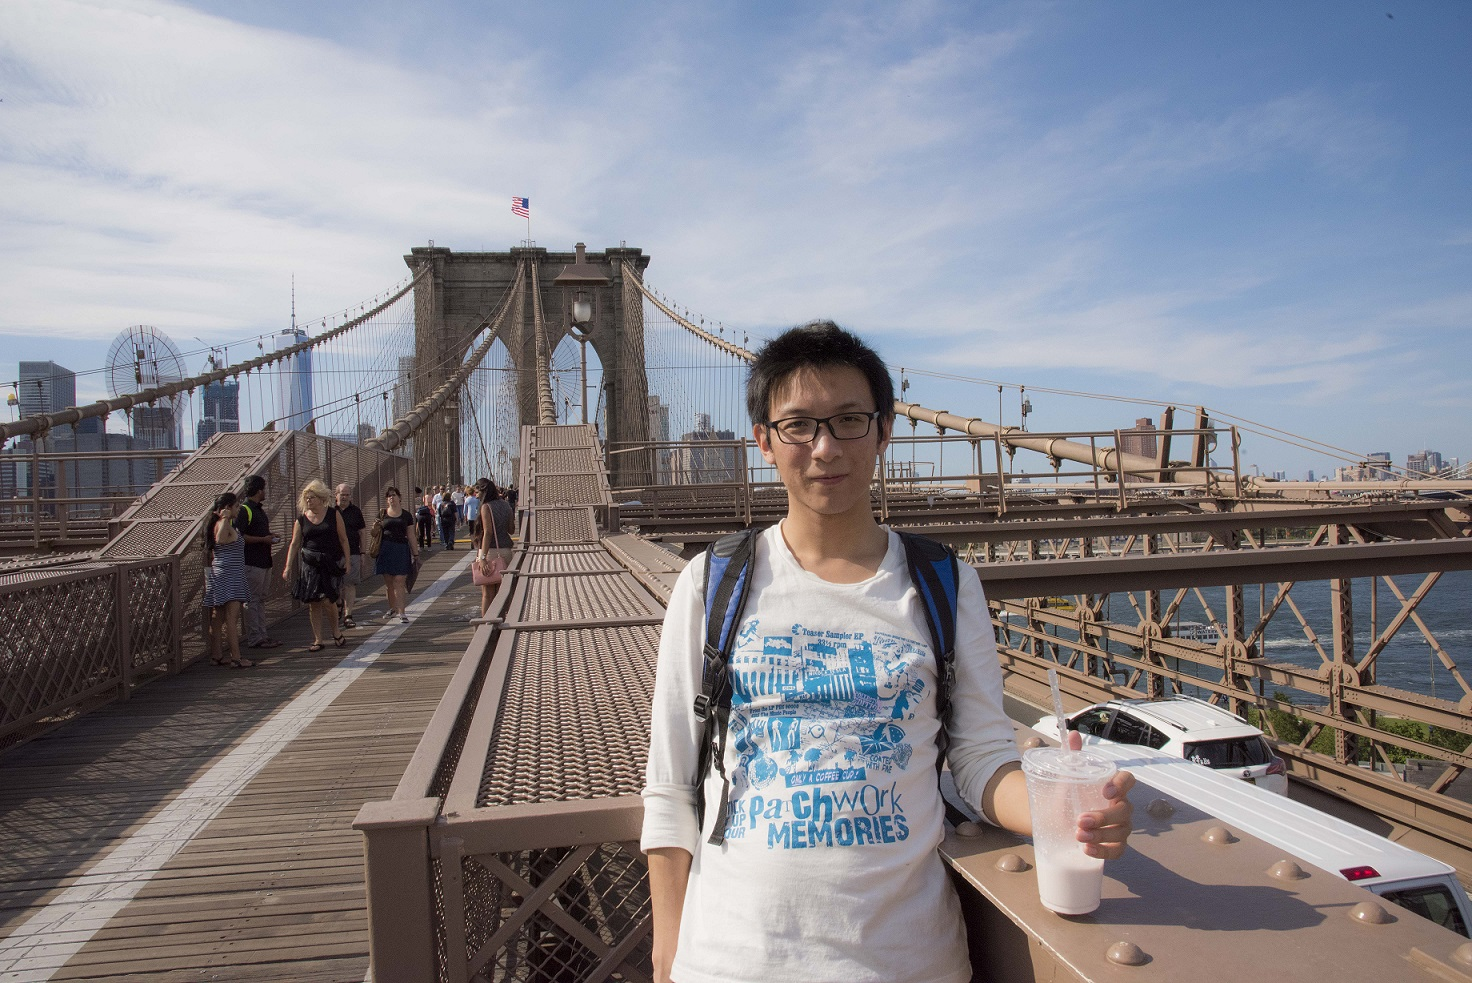
\includegraphics[height=4in]{brooklyn.jpg}

\end{document}

